\documentclass{article}

\usepackage{fancyhdr}
\usepackage{lastpage}
\usepackage{extramarks}
\usepackage[usenames,dvipsnames]{color}
\usepackage{amsmath}
\usepackage{amsthm}
\usepackage{amsfonts}
\usepackage{tikz}

\usetikzlibrary{automata,positioning,calc}

\topmargin=-0.45in
\evensidemargin=0in
\oddsidemargin=0in
\textwidth=6.5in
\textheight=9.0in
\headsep=0.25in

\linespread{1.1}

\pagestyle{fancy}
\lhead{\hmwkAuthorName}
\chead{\hmwkClass\ (\hmwkClassInstructor\ \hmwkClassTime): \hmwkTitle}
\rhead{\firstxmark}
\lfoot{\lastxmark}
\cfoot{}
\renewcommand\headrulewidth{0.4pt}
\renewcommand\footrulewidth{0.4pt}

\setlength\parindent{0pt}

\newcommand{\enterProblemHeader}[1]{
    \nobreak\extramarks{#1}{#1 continued on next page\ldots}\nobreak
    \nobreak\extramarks{#1 (continued)}{#1 continued on next page\ldots}\nobreak
}

\newcommand{\exitProblemHeader}[1]{
    \nobreak\extramarks{#1 (continued)}{#1 continued on next page\ldots}\nobreak
    \nobreak\extramarks{#1}{}\nobreak
}

\setcounter{secnumdepth}{0}
\newcounter{homeworkProblemCounter}

\newcommand{\homeworkProblemName}{}
\newenvironment{homeworkProblem}[1][Problem \arabic{homeworkProblemCounter}]{
    \stepcounter{homeworkProblemCounter}
    \renewcommand{\homeworkProblemName}{#1}
    \section{\homeworkProblemName}
    \enterProblemHeader{\homeworkProblemName}
}{
    \exitProblemHeader{\homeworkProblemName}
}

\newcommand{\problemAnswer}[1]{
\noindent\framebox[\columnwidth][c]{\begin{minipage}{0.98\columnwidth}#1\end{minipage}}
}

\newcommand{\homeworkSectionName}{}
\newenvironment{homeworkSection}[1]{
    \renewcommand{\homeworkSectionName}{#1}
    \subsection{\homeworkSectionName}
    \enterProblemHeader{\homeworkProblemName\ [\homeworkSectionName]}
}{
    \enterProblemHeader{\homeworkProblemName}
}

\newcommand{\hmwkTitle}{Homework\ \#5}
\newcommand{\hmwkDueDate}{March 07, 2013 at 11:59pm}
\newcommand{\hmwkClass}{CS331}
\newcommand{\hmwkClassTime}{9:00am}
\newcommand{\hmwkClassInstructor}{Professor Zhang}
\newcommand{\hmwkAuthorName}{Josh Davis}

\title{
    \vspace{2in}
    \textmd{\textbf{\hmwkClass:\ \hmwkTitle}}\\
    \normalsize\vspace{0.1in}\small{Due\ on\ \hmwkDueDate}\\
    \vspace{0.1in}\large{\textit{\hmwkClassInstructor\ \hmwkClassTime}}
    \vspace{3in}
}

\author{\textbf{\hmwkAuthorName}}
\date{}

\begin{document}

\maketitle

\pagebreak

\begin{homeworkProblem}
    Let \(\Sigma = \{0, 1\}\). Consider the following language over \(\Sigma\),
    \( L = \{w \in \Sigma^* : w \mbox{ contains twice as many 0's as 1's }\} \)
    \\

    \textbf{Part One} Describe in pseudo-code a Turing machine, \(M\) that recognizes \(L\).
    \\

    The pseudo-code that describes \(M\) is as follows:

    \(M = \)`` On input string \(w\):
    \begin{enumerate}
        \item Start on the left side of the word, move right until we find a 1, cross it out
        \item If in stage 1 and the tape is empty, mopve to \(q_{accept}\)
        \item If in stage 1 and we reach the end of the tape, move to \(q_{reject}\)
        \item Move back to the left of the word
        \item Scan right until a 0 is found, cross it out
        \item Move back to the left of the word
        \item If in previous stage and we reach the end of the tape, move to \(q_{reject}\)
        \item Scan right again until a 0 is found, cross it out
        \item Move to the left of the word
        \item If in previous stage and we reach the end of the tape, move to \(q_{reject}\)
        \item Move to left of the word, move to stage 1
    \end{enumerate}

    \textbf{Part Two} Formally define \(M\), where \(M = \langle \Sigma, \Gamma, Q, q_0, q_{accept}, q_{reject} \rangle\)
    \\

    \(M\) can be formally defined as follows:
    \begin{enumerate}
        \item \(\Gamma = \Sigma \cup \{\textvisiblespace, x\}\)
        \item \(Q = \{q_0, q_1, q_{accept}, q_{reject}\}\), the states
        \item \(q_0\), the start state
        \item Then \(\delta\) as given by the table:
            \begin{table}[ht]
                \centering
                \begin{tabular}{c || c | c | c | c}
                    \(\delta\) & 0 & 1 & x & \textvisiblespace \\
                    \hline
                    \(q_0\) & \((q_0, 0, R)\) & \((q_0, 1, R)\) & \((q_0, 0, R)\) & \((q_0, 0, R)\) \\
                    \(q_1\) & \((q_0, 0, R)\) & \((q_0, 1, R)\) & \((q_0, 0, R)\) & \((q_0, 0, R)\) \\
                    \(q_2\) & \((q_0, 0, R)\) & \((q_0, 1, R)\) & \((q_0, 0, R)\) & \((q_0, 0, R)\) \\
                    \(q_3\) & \((q_0, 0, R)\) & \((q_0, 1, R)\) & \((q_0, 0, R)\) & \((q_0, 0, R)\) \\
                    \(q_4\) & \((q_0, 0, R)\) & \((q_0, 1, R)\) & \((q_0, 0, R)\) & \((q_0, 0, R)\) \\
                    \(q_5\) & \((q_0, 0, R)\) & \((q_0, 1, R)\) & \((q_0, 0, R)\) & \((q_0, 0, R)\) \\
                    \(q_6\) & \((q_0, 0, R)\) & \((q_0, 1, R)\) & \((q_0, 0, R)\) & \((q_0, 0, R)\) \\
                    \(q_7\) & \((q_0, 0, R)\) & \((q_0, 1, R)\) & \((q_0, 0, R)\) & \((q_0, 0, R)\) \\
                    \(q_8\) & \((q_0, 0, R)\) & \((q_0, 1, R)\) & \((q_0, 0, R)\) & \((q_0, 0, R)\) \\
                    \(q_9\) & \((q_0, 0, R)\) & \((q_0, 1, R)\) & \((q_0, 0, R)\) & \((q_0, 0, R)\) \\
                    \(q_{10}\) & \((q_0, 0, R)\) & \((q_0, 1, R)\) & \((q_0, 0, R)\) & \((q_0, 0, R)\) \\
                \end{tabular}
            \end{table}
    \end{enumerate}

\end{homeworkProblem}

\pagebreak

\begin{homeworkProblem}
    Let \(\Sigma = \{0, 1\}\) and \(\Gamma = \{0, 1, \textvisiblespace, \#, x\}\). Write a Turing machine, \(M\),
    such that given any input \(w \in \Sigma^*\), \(M\) halts with tape content \(w\#w^R\).
    \\

    \textbf{Part One} Describe \(M\) in pseudo-code.
    \\

    That pseudo-code that describes \(M\) is as follows:
    \(M = \)" On input string \(w\):
    \begin{enumerate}
        \item Start on left side of the input, move right until no 0 or 1 is found
            mark the tape with \#
        \item 
    \end{enumerate}
    "

    \textbf{Part Two} Formally define \(M\)
    \\



\end{homeworkProblem}

\pagebreak

\begin{homeworkProblem}
    Let \(M = \langle \Sigma, \Gamma, Q, q_0, \delta, q_{accept}, q_{reject}
    \rangle \) be a Turing machine where \(\Sigma = \{0, 1\}\), \(\Gamma = \{0, 1, \textvisiblespace \}\),

    \(Q = \{q_0, q_1, q_2, q_3, q_{accept}, q_{reject}\}\) and \(\delta\) is represented by the
    following table:

    \begin{table}[ht]
        \centering
        \begin{tabular}{c || c | c | c | c}
            \(\delta\) & 0 & 1 & \textvisiblespace \\
            \hline
            \(q_0\) & \((q_0, 0, R)\) & \((q_0, 1, R)\) & \((q_1, \textvisiblespace, L)\) \\
            \(q_1\) & \((q_2, 1, L)\) & \((q_1, 0, L)\) & \((q_3, 1, L)\) \\
            \(q_2\) & \((q_2, 0, L)\) & \((q_1, 1, L)\) & \((q_{accept}, \textvisiblespace, R)\) \\
            \(q_3\) & - & - & \((q_{accept}, \textvisiblespace, R)\) \\
        \end{tabular}
    \end{table}

    \textbf{Part One} Show the sequence of computation of \(M\) when given 01101 input.
    \\

    Read from left to right, top to bottom, the sequence is as follows:
    \begin{figure}[h]
        \centering
        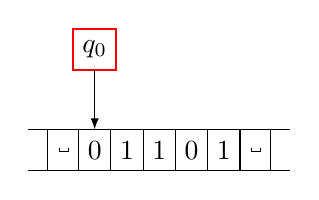
\begin{tikzpicture}[every node/.style={block}, block/.style={minimum height=1.5em,outer sep=0pt,draw,rectangle,node distance=0pt}]
            \node (C) {$1$};
            \node (B) [left=of C] {$1$};
            \node (A) [left=of B] {$0$};
            \node (0) [left=of A] {$\textvisiblespace$};
            \node (D) [right=of C] {$0$};
            \node (E) [right=of D] {$1$};
            \node (1) [right=of E] {$\textvisiblespace$};
            \node (F) [above = 0.75cm of A,draw=red,thick] {$q_0$};
            \draw[-latex] (F) -- (A);
            \draw (0.north west) -- ++(-.25cm,0) (0.south west) -- ++ (-.25cm,0) 
                (1.north east) -- ++(.25cm,0) (1.south east) -- ++ (.25cm,0);
        \end{tikzpicture}
        \hspace{20px}
        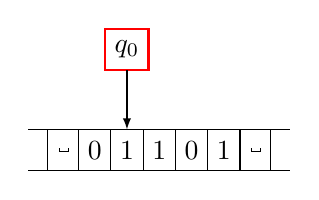
\begin{tikzpicture}[every node/.style={block}, block/.style={minimum height=1.5em,outer sep=0pt,draw,rectangle,node distance=0pt}]
            \node (C) {$1$};
            \node (B) [left=of C] {$1$};
            \node (A) [left=of B] {$0$};
            \node (0) [left=of A] {$\textvisiblespace$};
            \node (D) [right=of C] {$0$};
            \node (E) [right=of D] {$1$};
            \node (1) [right=of E] {$\textvisiblespace$};
            \node (F) [above = 0.75cm of B,draw=red,thick] {$q_0$};
            \draw[-latex] (F) -- (B);
            \draw (0.north west) -- ++(-.25cm,0) (0.south west) -- ++ (-.25cm,0) 
                (1.north east) -- ++(.25cm,0) (1.south east) -- ++ (.25cm,0);
        \end{tikzpicture}
        \hspace{20px}
        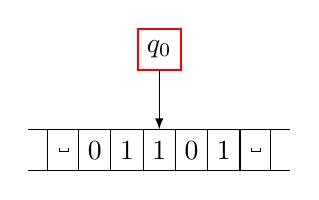
\begin{tikzpicture}[every node/.style={block}, block/.style={minimum height=1.5em,outer sep=0pt,draw,rectangle,node distance=0pt}]
            \node (C) {$1$};
            \node (B) [left=of C] {$1$};
            \node (A) [left=of B] {$0$};
            \node (0) [left=of A] {$\textvisiblespace$};
            \node (D) [right=of C] {$0$};
            \node (E) [right=of D] {$1$};
            \node (1) [right=of E] {$\textvisiblespace$};
            \node (F) [above = 0.75cm of C,draw=red,thick] {$q_0$};
            \draw[-latex] (F) -- (C);
            \draw (0.north west) -- ++(-.25cm,0) (0.south west) -- ++ (-.25cm,0) 
                (1.north east) -- ++(.25cm,0) (1.south east) -- ++ (.25cm,0);
        \end{tikzpicture}
        \hspace{20px}
        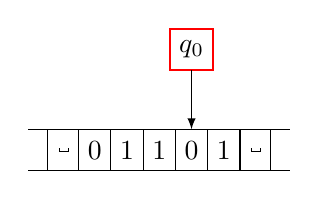
\begin{tikzpicture}[every node/.style={block}, block/.style={minimum height=1.5em,outer sep=0pt,draw,rectangle,node distance=0pt}]
            \node (C) {$1$};
            \node (B) [left=of C] {$1$};
            \node (A) [left=of B] {$0$};
            \node (0) [left=of A] {$\textvisiblespace$};
            \node (D) [right=of C] {$0$};
            \node (E) [right=of D] {$1$};
            \node (1) [right=of E] {$\textvisiblespace$};
            \node (F) [above = 0.75cm of D,draw=red,thick] {$q_0$};
            \draw[-latex] (F) -- (D);
            \draw (0.north west) -- ++(-.25cm,0) (0.south west) -- ++ (-.25cm,0) 
                (1.north east) -- ++(.25cm,0) (1.south east) -- ++ (.25cm,0);
        \end{tikzpicture}

        \vspace{20px}

        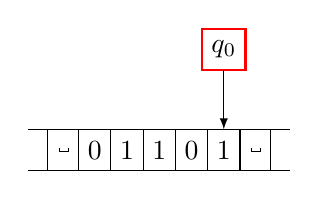
\begin{tikzpicture}[every node/.style={block}, block/.style={minimum height=1.5em,outer sep=0pt,draw,rectangle,node distance=0pt}]
            \node (C) {$1$};
            \node (B) [left=of C] {$1$};
            \node (A) [left=of B] {$0$};
            \node (0) [left=of A] {$\textvisiblespace$};
            \node (D) [right=of C] {$0$};
            \node (E) [right=of D] {$1$};
            \node (1) [right=of E] {$\textvisiblespace$};
            \node (F) [above = 0.75cm of E,draw=red,thick] {$q_0$};
            \draw[-latex] (F) -- (E);
            \draw (0.north west) -- ++(-.25cm,0) (0.south west) -- ++ (-.25cm,0) 
                (1.north east) -- ++(.25cm,0) (1.south east) -- ++ (.25cm,0);
        \end{tikzpicture}
        \hspace{20px}
        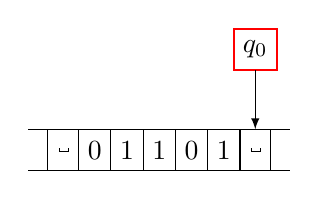
\begin{tikzpicture}[every node/.style={block}, block/.style={minimum height=1.5em,outer sep=0pt,draw,rectangle,node distance=0pt}]
            \node (C) {$1$};
            \node (B) [left=of C] {$1$};
            \node (A) [left=of B] {$0$};
            \node (0) [left=of A] {$\textvisiblespace$};
            \node (D) [right=of C] {$0$};
            \node (E) [right=of D] {$1$};
            \node (1) [right=of E] {$\textvisiblespace$};
            \node (F) [above = 0.75cm of 1,draw=red,thick] {$q_0$};
            \draw[-latex] (F) -- (1);
            \draw (0.north west) -- ++(-.25cm,0) (0.south west) -- ++ (-.25cm,0) 
                (1.north east) -- ++(.25cm,0) (1.south east) -- ++ (.25cm,0);
        \end{tikzpicture}
        \hspace{20px}
        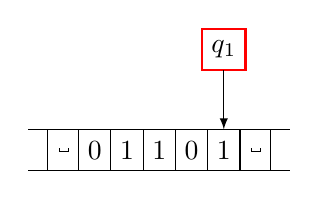
\begin{tikzpicture}[every node/.style={block}, block/.style={minimum height=1.5em,outer sep=0pt,draw,rectangle,node distance=0pt}]
            \node (C) {$1$};
            \node (B) [left=of C] {$1$};
            \node (A) [left=of B] {$0$};
            \node (0) [left=of A] {$\textvisiblespace$};
            \node (D) [right=of C] {$0$};
            \node (E) [right=of D] {$1$};
            \node (1) [right=of E] {$\textvisiblespace$};
            \node (F) [above = 0.75cm of E,draw=red,thick] {$q_1$};
            \draw[-latex] (F) -- (E);
            \draw (0.north west) -- ++(-.25cm,0) (0.south west) -- ++ (-.25cm,0) 
                (1.north east) -- ++(.25cm,0) (1.south east) -- ++ (.25cm,0);
        \end{tikzpicture}
        \hspace{20px}
        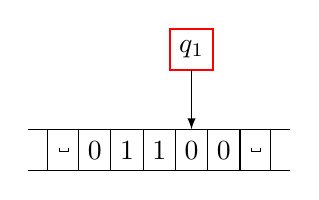
\begin{tikzpicture}[every node/.style={block}, block/.style={minimum height=1.5em,outer sep=0pt,draw,rectangle,node distance=0pt}]
            \node (C) {$1$};
            \node (B) [left=of C] {$1$};
            \node (A) [left=of B] {$0$};
            \node (0) [left=of A] {$\textvisiblespace$};
            \node (D) [right=of C] {$0$};
            \node (E) [right=of D] {$0$};
            \node (1) [right=of E] {$\textvisiblespace$};
            \node (F) [above = 0.75cm of D,draw=red,thick] {$q_1$};
            \draw[-latex] (F) -- (D);
            \draw (0.north west) -- ++(-.25cm,0) (0.south west) -- ++ (-.25cm,0) 
                (1.north east) -- ++(.25cm,0) (1.south east) -- ++ (.25cm,0);
        \end{tikzpicture}

        \vspace{20px}

        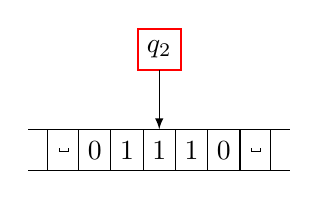
\begin{tikzpicture}[every node/.style={block}, block/.style={minimum height=1.5em,outer sep=0pt,draw,rectangle,node distance=0pt}]
            \node (C) {$1$};
            \node (B) [left=of C] {$1$};
            \node (A) [left=of B] {$0$};
            \node (0) [left=of A] {$\textvisiblespace$};
            \node (D) [right=of C] {$1$};
            \node (E) [right=of D] {$0$};
            \node (1) [right=of E] {$\textvisiblespace$};
            \node (F) [above = 0.75cm of C,draw=red,thick] {$q_2$};
            \draw[-latex] (F) -- (C);
            \draw (0.north west) -- ++(-.25cm,0) (0.south west) -- ++ (-.25cm,0) 
                (1.north east) -- ++(.25cm,0) (1.south east) -- ++ (.25cm,0);
        \end{tikzpicture}
        \hspace{20px}
        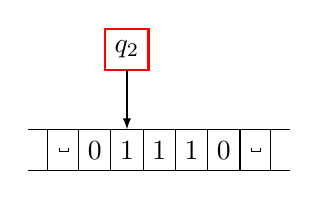
\begin{tikzpicture}[every node/.style={block}, block/.style={minimum height=1.5em,outer sep=0pt,draw,rectangle,node distance=0pt}]
            \node (C) {$1$};
            \node (B) [left=of C] {$1$};
            \node (A) [left=of B] {$0$};
            \node (0) [left=of A] {$\textvisiblespace$};
            \node (D) [right=of C] {$1$};
            \node (E) [right=of D] {$0$};
            \node (1) [right=of E] {$\textvisiblespace$};
            \node (F) [above = 0.75cm of B,draw=red,thick] {$q_2$};
            \draw[-latex] (F) -- (B);
            \draw (0.north west) -- ++(-.25cm,0) (0.south west) -- ++ (-.25cm,0) 
                (1.north east) -- ++(.25cm,0) (1.south east) -- ++ (.25cm,0);
        \end{tikzpicture}
        \hspace{20px}
        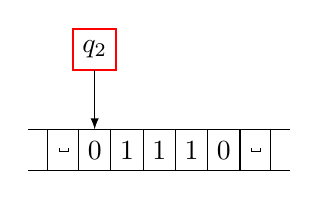
\begin{tikzpicture}[every node/.style={block}, block/.style={minimum height=1.5em,outer sep=0pt,draw,rectangle,node distance=0pt}]
            \node (C) {$1$};
            \node (B) [left=of C] {$1$};
            \node (A) [left=of B] {$0$};
            \node (0) [left=of A] {$\textvisiblespace$};
            \node (D) [right=of C] {$1$};
            \node (E) [right=of D] {$0$};
            \node (1) [right=of E] {$\textvisiblespace$};
            \node (F) [above = 0.75cm of A,draw=red,thick] {$q_2$};
            \draw[-latex] (F) -- (A);
            \draw (0.north west) -- ++(-.25cm,0) (0.south west) -- ++ (-.25cm,0) 
                (1.north east) -- ++(.25cm,0) (1.south east) -- ++ (.25cm,0);
        \end{tikzpicture}
        \hspace{20px}
        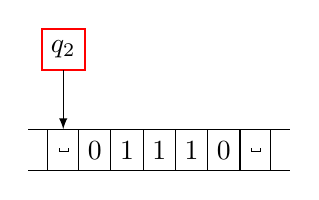
\begin{tikzpicture}[every node/.style={block}, block/.style={minimum height=1.5em,outer sep=0pt,draw,rectangle,node distance=0pt}]
            \node (C) {$1$};
            \node (B) [left=of C] {$1$};
            \node (A) [left=of B] {$0$};
            \node (0) [left=of A] {$\textvisiblespace$};
            \node (D) [right=of C] {$1$};
            \node (E) [right=of D] {$0$};
            \node (1) [right=of E] {$\textvisiblespace$};
            \node (F) [above = 0.75cm of 0,draw=red,thick] {$q_2$};
            \draw[-latex] (F) -- (0);
            \draw (0.north west) -- ++(-.25cm,0) (0.south west) -- ++ (-.25cm,0) 
                (1.north east) -- ++(.25cm,0) (1.south east) -- ++ (.25cm,0);
        \end{tikzpicture}
        
        \vspace{20px}

        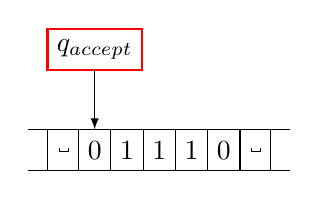
\begin{tikzpicture}[every node/.style={block}, block/.style={minimum height=1.5em,outer sep=0pt,draw,rectangle,node distance=0pt}]
            \node (C) {$1$};
            \node (B) [left=of C] {$1$};
            \node (A) [left=of B] {$0$};
            \node (0) [left=of A] {$\textvisiblespace$};
            \node (D) [right=of C] {$1$};
            \node (E) [right=of D] {$0$};
            \node (1) [right=of E] {$\textvisiblespace$};
            \node (F) [above = 0.75cm of A,draw=red,thick] {$q_{accept}$};
            \draw[-latex] (F) -- (A);
            \draw (0.north west) -- ++(-.25cm,0) (0.south west) -- ++ (-.25cm,0) 
                (1.north east) -- ++(.25cm,0) (1.south east) -- ++ (.25cm,0);
        \end{tikzpicture}
    \end{figure}

    \textbf{Part Two} What is the functionality of \(M\)? Justify your answer.
    \\

    Given a word that represents a number in binary, it will increment it based
    on the rules of binary addition.
    \\

    \textbf{Justification}
    \\

    In binary addition a 1 is added to the farthest right place value of
    the number. If this value is 1, it will flip it to 0 and carry to the next
    place value to the left.
    \\

    This flipping will occur until a 0 is reached or the read/write head reaches the end
    of the number. It will then flip the 0 to a 1, or the space to a 1.
    \\

    The result is that the binary representation of the number will be incremented.
\end{homeworkProblem}

\pagebreak

\begin{homeworkProblem}
    Use pumping lemma to show that the following language is not context-free:
    \[
        L = \{a^i b^j c^k : i, j, k \geq 0 \mbox{ and } i > j \mbox{ and } j > k \}
    \]

    \begin{proof}
        We let \(w = a^{p + 2} b^{p + 1} c^{p}\) where \(p\) is the pumping length.
        We then split up \(w\) so that \(w = uvxyz\). In doing so, we can break it up into
        cases like so:
        \begin{enumerate}
            \item \(vxy\) contains just a's. This will result in a contradiction
                because pumping down yields \(a^{0} a^{p - 2} a^{0} = \epsilon a^p \epsilon\) which means \(i \leq j\) and
                thus \(w \notin L\).
            \item \(vxy\) contains just b's. This will result in a contradiction
                because pumping down yields \(b^{0} b^{p - 2} b^{0} = \epsilon b^p \epsilon\) which means \(j \leq k\) and
                thus \(w \notin L\).
            \item \(vxy\) contains just c's. This will result in a contradiction
                because pumping up will eventually give us \(k > j\)
                thus \(w \notin L\).
            \item \(vxy\) is the split between a's and b's. 
                This can be divided into four more cases:
                \begin{enumerate}
                    \item \(vxy = aab\), pumping down will lower the number of b's to be the same as
                        the number of c's. Thus \(w \notin L\).
                    \item \(vxy = abb\), pumping down will lower the number of a's to be the same as
                        the number of b's. Thus \(w \notin L\).
                    \item \(vxy = \epsilon ab\), pumping up will increase the number of b's past the
                        number of a's. Thus \(w \notin L\).
                    \item \(vxy = ab \epsilon\), pumping down will lower the number of a's to be the
                        same as the number of b's. Thus \(w \notin L\).
                \end{enumerate}

            \item \(vxy\) is the split between b's and c's. Regardless of where the subsplit is,
                it can be pumped until eventually \(i < j\) or \(i < k\), thus \(w \notin L\).
        \end{enumerate}

        Now that I have (hopefully) exhausted all possibilities, the proof is complete and the language,
        \(L\), is not context-free.
    \end{proof}
\end{homeworkProblem}

\pagebreak

\begin{homeworkProblem}
    Let \(G = \langle \{S\}, \{a, b\}, R, S \rangle\) be a context-free grammar
    with the rules, \(R\) defined as follows:
    \[
        S \rightarrow aS | aSbS | \epsilon
    \]

    \textbf{Part One}
    Prove that \(G\) is ambiguous.
    \\
    \begin{proof}
        We can prove that \(G\) is ambiguous if there are two left most derivations
        for one string.
        \\

        Take \(s = aab\), it can be derived twice as follows:
        \[
            \begin{split}
                S &= aS = aaSbS = aabS = aab
                \\
                S &= aSbS = aaSbS = aabS = aab
            \end{split}
        \]

        Thus the context free language, \(G\) is ambiguous.
    \end{proof}

    \textbf{Part Two}
    Give unambigous grammar that generates the same language as \(G\).
    \\

    The new grammar can be defined as follows:
    \[
        \begin{split}
            S &\rightarrow aT | T
            \\
            T &\rightarrow aSbU | S
            \\
            U &\rightarrow a | b | \epsilon
        \end{split}
    \]

    Using the previous example of \(s = aab\), we can try to derive it multiple times
    like so:
    \[
        \begin{split}
            S &= aT = aSbU = aTbU = aabU = aab
            \\
            S &= T = aSbU = ... = \mbox{ no way to get aab}
        \end{split}
    \]

    And there it can't be derived multiple ways. So unless I'm missing
    something, I think the homework is finished. YAY!

\end{homeworkProblem}

\end{document}
